\section{Backend}
Als Technologie für die Implementierung des Backends wird das Asp.Net Core Framework von Microsoft eingesetzt. Grund dafür ist, dass alle benötigten Funktionen wie Webfrontends, REST APIs oder Identity Management nativ und gleichzeitig plattformunabhängig unterstützt werden. Als Programmiersprache wird C\# eingesetzt.

\subsection{Authentifizierung und Autorisierung}
Für die Umsetzung der Benutzerauthentifizierung und die Rechteverwaltung wird IdentityServer4\footnote{\url{http://docs.identityserver.io/en/release/}} eingesetzt. Dieses Framework erlaubt eine moderne zentralisierte Identitätsverwaltung für verschiedene Anwendungsszenarien basierend auf OpenId und OAuth2. 

\begin{figure}[h]
  \begin{center}
    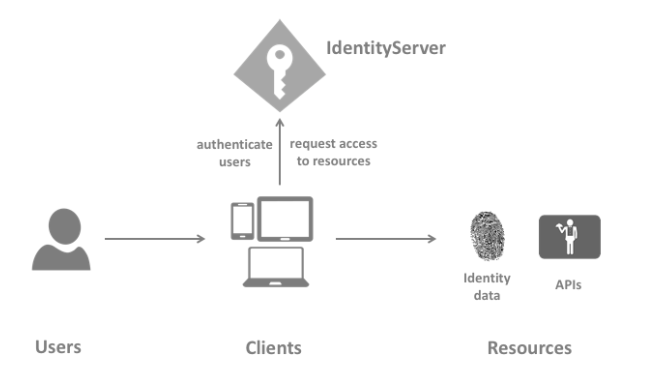
\includegraphics[width=\textwidth]{./img/BackendIdentityServer.png}
    \caption{Terminologien des Identity Servers}
    \label{fig:backendIdentityServer}
  \end{center}
\end{figure}

Das Grundkonzept des Identity Servers wird in Abbildung \ref{fig:backendIdentityServer} gezeigt. \textbf{Benutzer} greifen dabei über verschiedene \textbf{Clients} auf geschützt \textbf{Ressourcen} wie APIs oder Anwendungsbereiche zu, die von dem Identitätsserver geschützt werden. Dieses Konzept passt auf das in diesem Projekt entstehende Szenario, in dem Benutzer entweder über die Smartphone App oder das Webfrontend des Backends (Clients) auf die Web API zugreifen (Ressource).

\begin{figure}[h]
  \begin{center}
    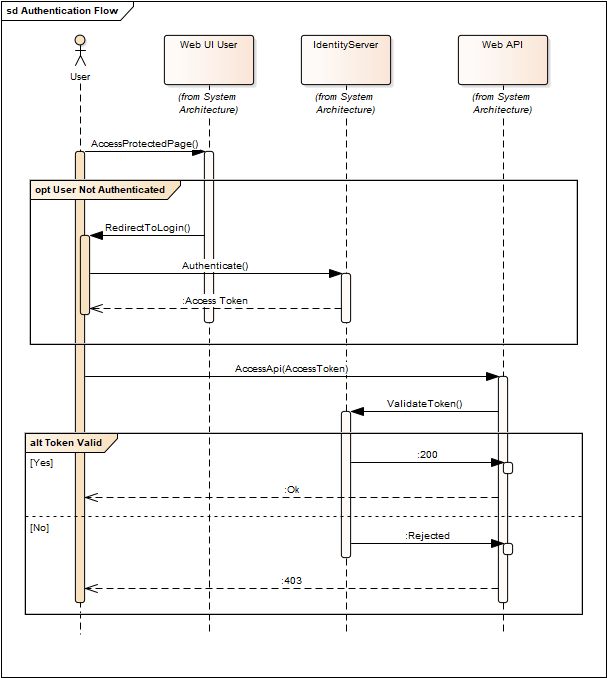
\includegraphics[width=\textwidth]{./img/BackendAuthenticationFlow.png}
    \caption{Ablauf der Authentifizierung beim Zugriff auf geschützte Ressourcen}
    \label{fig:backendAuthenticationFlow}
  \end{center}
\end{figure}

Der implementierte Ablauf der Authentifizierung erfolgt nach dem in Abbildung \ref{fig:backendAuthenticationFlow} skizzierten Schema. Beim Zugriff auf eine geschützte Funktion im Web UI wird der Benutzer auf die Login Seite des Identity Servers weitergeleitet, wo er sich entweder registrieren oder einloggen kann. Nach erfolgreicher Authentifizierung generiert der Identity Server ein Access Token, welches in der Session des Benutzers gespeichert wird und Informationen über den Benutzer, die für ihn freigegebenen Ressourcen sowie die dem Nutzer zugeordneten Claims enthält. Bei einem anschließenden Zugriff die Web API wird dieses Token mitgeschickt und von der API beim Identity Server validiert.

\subsection{Datenbank und Zugriff}
Als Datenbank wird MySql eingesetzt da es einfach in der Anwendung und schlank im Betrieb ist. Als alternative wurde ebenfalls Sql Server evaluiert, was den Vorteil der besseren Integration in die Asp.Net Core Umgebung gehabt hätte. Der zugehörige Docker Container (vgl. \ref{sec:backendDeployment}) hat jedoch 4GB Arbeitsspeicher erfordert, was zusätzlich zum normalen Betriebssystem und der Entwicklungsumgebung mehr als die momentan üblicherweise verbauten 8GB \ac{RAM} übertrifft.

Der Zugriff auf die Datenbank erfolgt nicht direkt über SQL-Anfragen sondern über Entity Framework, ein Framework für objektrelationale Abbildung. Dabei werden die Daten im Hintergrund in Collections geladen, sodass es für den Benutzer aussieht, als würden die Daten direkt im RAM liegen. Dieses System bietet - insbesondere in Kombination mit \ac{LINQ} in C\#- den Vorteil, dass der Code wesentlich übersichtlicher und leichter verständlich wird, da das direkte Laden der Daten mittels SQL-Anfragen und anschließendem manuellen einlesen entfällt.

Für die Integration von Entity Framework für MySql Datenbanken in einer Asp.Net Core Umgebung muss ein Third Party NuGet Paket\footnote{\url{https://www.nuget.org/packages/Pomelo.EntityFrameworkCore.MySql}} verwendet werden, da zum Zeitpunkt der Entwicklung keine native Anbindung zur Verfügung steht. Das verwendete Paket hat allerdings Performanceprobleme bei der Verarbeitung größerer Datenmengen. Schon das speichern und laden von Fahrten mit einer Rohdatenmenge von ~500kB führen zu Verzögerungen von ca. 30 Sekunden. Die einzig verbleibende Alternative um das Problem zu beheben ist der Austausch der Datenbank, wozu während der Projektlaufzeit keine Ressourcen mehr zur Verfügung stehen.

\subsection{Bereitstellung}
\label{sec:backendDeployment}
Da das Backend aus verschiedenen zunächst unabhängigen Komponenten besteht und einige Voraussetzungen bezüglich der Infrastruktur mit sich bringt, ist die Bereitstellung einer Produktivumgebung nicht trivial. 
Aus diesem Grund wird die Containervirtualisierung Docker eingesetzt, um das Gesamtsystem leicht installierbar zu machen.

Docker\footnote{\url{https://docs.docker.com/}} unterscheidet von normalen virtuellen Maschinen darin, dass nicht für jede Instanz ein gesamtes Hostsystem emuliert wird, sonder lediglich die Applikation samt ihrer Abhängigkeiten in dem Container stecken. In der Terminologie wird bei Docker zwischen Containern und Images unterschieden. Ein Image ist dabei ein Speicherabbild, aus dem heraus sich mehrere Container starten lassen (vergleichbar mit Klassen und Instanzen bei objektorientierter Programmierung). Für die Installation bedeutet das, dass nur die Images aller am System beteiligten Module zur Verfügung stehen müssen um aus jedem Image einen Container zu starten. Um das hochfahren komplexerer Anwendungen die aus mehreren Containern bestehen zu erleichtern, gibt es das Tool Docker Compose. Hiermit lassen sich verschiedene Parameter einstellen und alle Container gemeinsam starten was den Aufwand bei der Bereitstellung weiter reduziert. 

Um das SmartCar Backend in einer neuen Umgebung auszurollen werden lediglich die Images der Module, sowie das docker-compose File benötigt. Zusätzlich muss natürlich Docker auf dem Zielsystem installiert sein. Ist alles vorhanden, lässt sich über den Befehl \texttt{docker-compose up} die gesamte Umgebung ohne zusätzlichen Installationen hochfahren.


  

 
 
 
 
 
 
 
 